\documentclass[12pt]{article}
\usepackage{geometry}
\usepackage{amsmath}
\usepackage{mathtools}
\usepackage{amssymb}
\usepackage{enumitem}
\usepackage{fancyhdr}
\usepackage{tikz}
\usepackage{color}
\usepackage{xspace}
\usepackage{thumbpdf}
\usepackage{listings}
\usepackage{verbatim}
\usepackage{hyperref}
\usepackage{booktabs}
\usepackage{colortbl}
\usetikzlibrary{trees}
\usetikzlibrary{shapes,arrows}
\pagestyle{fancy}

\newcommand{\xref}[1]{\S\ref{#1}}
\definecolor{darkred}{rgb}{0.7,0,0}
\definecolor{darkgreen}{rgb}{0,0.5,0}
\hypersetup{colorlinks=true,
	linkcolor=darkred,
	citecolor=darkgreen}

\lstset{
	basicstyle=\ttfamily,
	mathescape
}

\lstdefinestyle{customc}{
	belowcaptionskip=1\baselineskip,
	breaklines=true,
	% xleftmargin=20pt,
	language=matlab,
	% frame=L,
	escapeinside={@}{@},
	showstringspaces=false,
	basicstyle=\small\ttfamily,
	keywordstyle=\bfseries\color{green!40!black},
	commentstyle=\itshape\color{purple!40!black},
	%identifierstyle=\color{blue},
	stringstyle=\color{orange},
	% directivestyle=\color{brown},
	%numbers=left,
	%numberstyle=\tiny\color{gray}
}

\lstdefinestyle{customctable}{
	aboveskip=-\medskipamount,
	belowskip=-\medskipamount,
	language=C,
	escapeinside={@}{@},
	showstringspaces=false,
	basicstyle=\scriptsize\ttfamily,
	keywordstyle=\bfseries\color{green!40!black},
	commentstyle=\itshape\color{purple!40!black},
	%identifierstyle=\color{blue},
	stringstyle=\color{orange},
	directivestyle=\color{brown},
}

\textheight=8.5in

\newcommand{\hongzi}[1]{{{\color{red}(HM: #1)}}}

\lhead{6.854 Pset 6}
\chead{Hongzi Mao \footnotesize{collaborators:} Calvin Lee, Linus Hamilton}
\rhead{Oct 19, 2016}

\begin{document}
	
\section*{Problem 1}
\paragraph{(a)} Suppose the cost of the edge $e(i,j)$ that we modified was originally $k$ and we decrease it to $k-1$. The other direction of increasing cost is similar in the sense that the reverse direction of the edge on the residual graph has the cost decreasing. Now we use BFS to find all paths from $j$ to $i$ with cost $-k$, the combination of each such path and the edge results in a negative cost cycle. 

Notice here that we only look for $-k$ cost. This is because, any path with total cost smaller than $-k$ (e.g. $-k-1$) can not exist, otherwise with the original cost $k$ in $e(i, j)$ it already results in a negative cost cycle and there is a smaller cost flow in the original graph, contradicts with the assumption that the flow is min-cost flow. For any path with total cost larger than $-k$, there is no need to push flow to the cycle, because the total cost along the cycle is non-negative.

After finding the paths using BFS, we invoke a max-flow algorithm to push as much flow as possible\footnote{An artificial source may be needed to bound the maximum possible flow from $j$ to $i$ by the residual amount of flow in $e(i, j)$.} \emph{only} on those paths in the residual graph, which results in a largest \emph{reduction} in the total cost, which still maintain the max flow in the scaled graph.  

Furthermore, notice that \emph{only} a single such operation is needed for the edge. This is because we will not introduce \emph{new} negative cost cycle after the flow augmentation. The reason is illustrated in Figure \ref{fig:1-1}. Suppose a new cycle is somehow created, with dashed arrows which are created in the residual graph after flow augmentation. Then the original graph must contain a path with smaller cost than $-k$, contradicts with the assertion we arrived. 
\begin{figure}[h!]
	\centering
	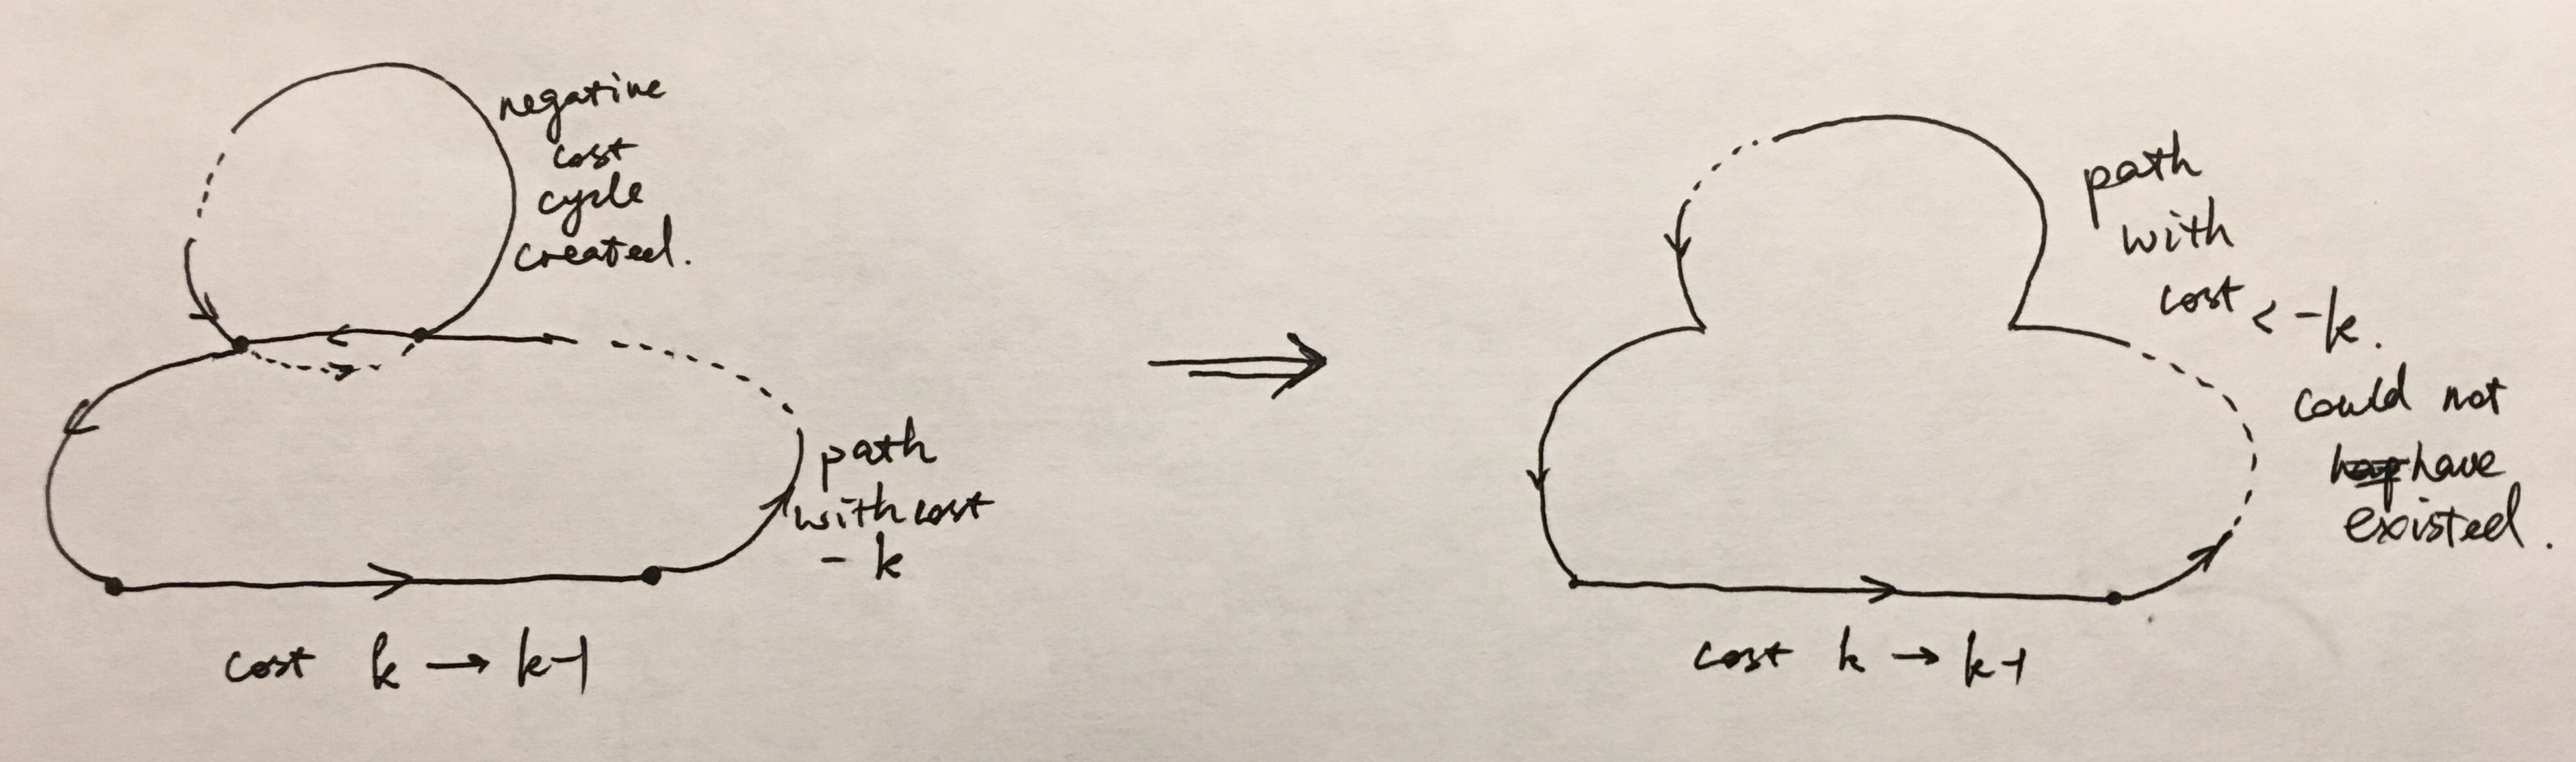
\includegraphics[width=1\textwidth]{1-1.jpg}
	\caption{Why \emph{only} a single such operation is needed for the modified edge.}
	\label{fig:1-1}
\end{figure}

In a more general case as Figure \ref{fig:1-2}, the new negative cost cycle and the path we pushed flow can be decomposed to an alternative path and (possible) cycles with smaller total cost, which contradicts with the assertion we made before. 

Therefore we only need to run plain max flow algorithm once on the paths we discovered using BFS. The BFS step takes $O(m)$ time and we can use the state of art algorithm with $\tilde{O}(mn)$ time bound.

\begin{figure}[h!]
\centering
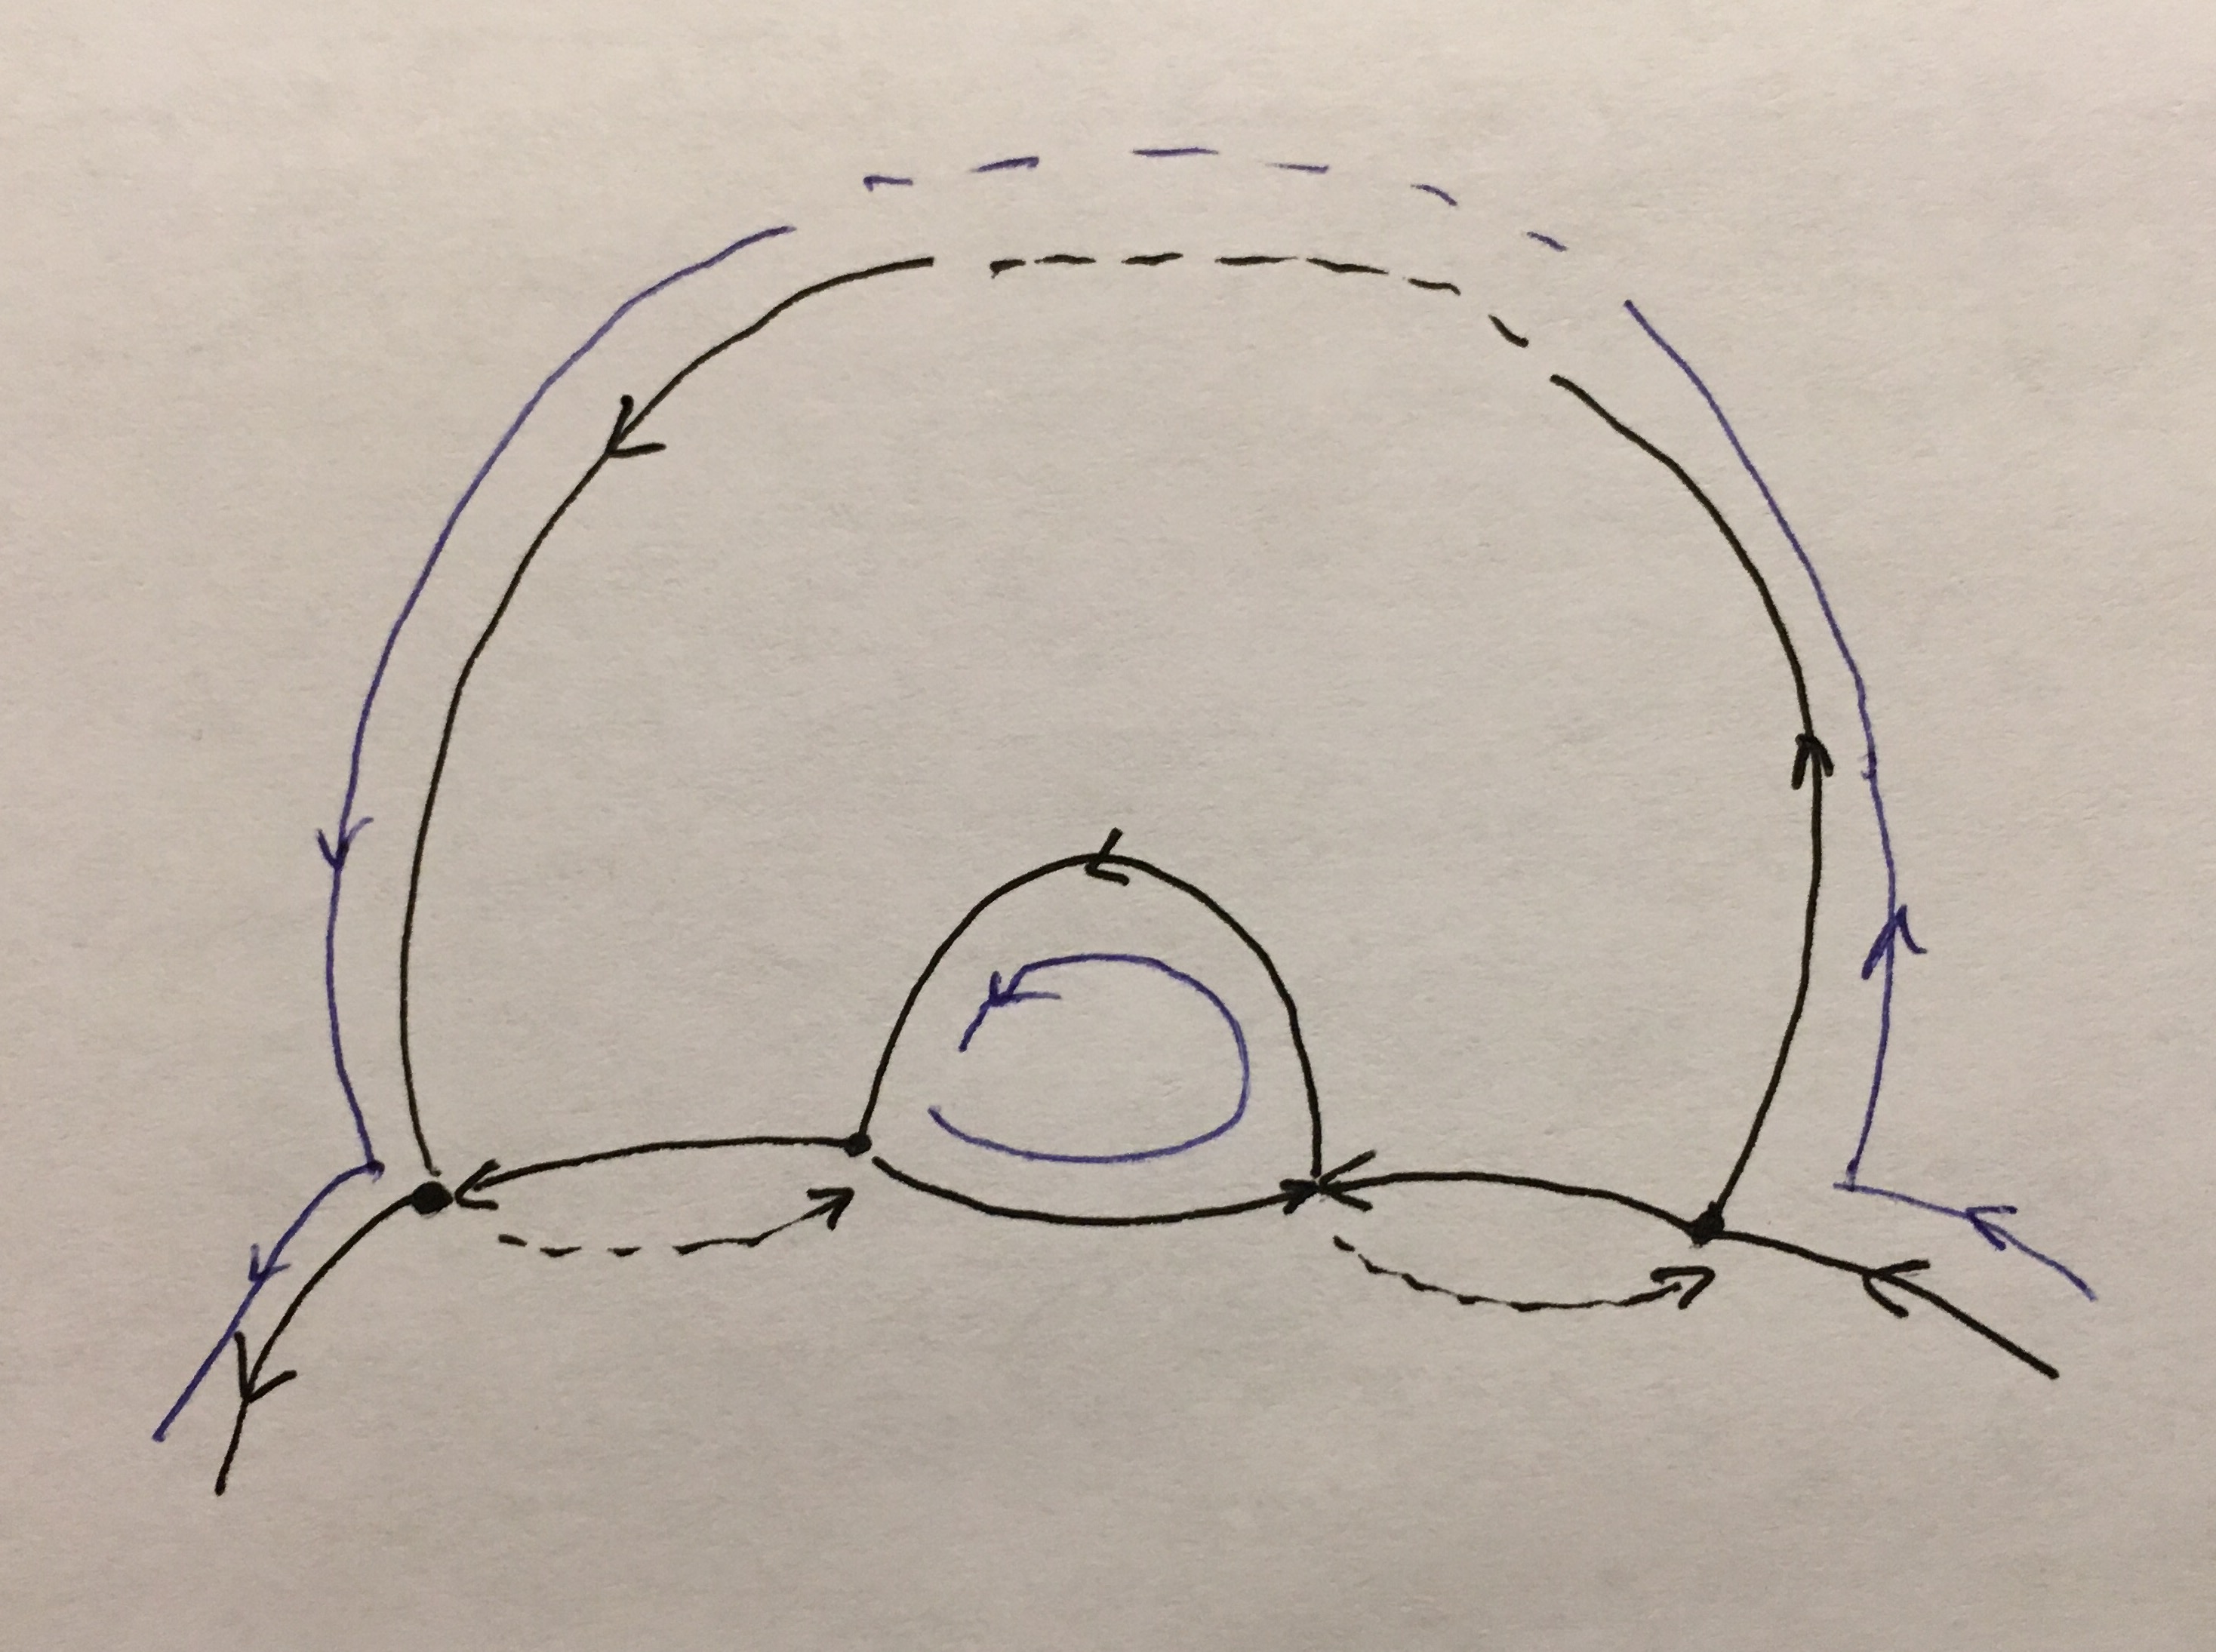
\includegraphics[width=0.5\textwidth]{1-2.jpg}
\caption{A more general case why \emph{only} a single such operation is needed for the modified edge. Decompose the path and a newly generated negative cost cycle (black), to another path with cycle(s) (blue).}
\label{fig:1-2}
\end{figure}
\paragraph{(b)} After each scaling, there are at most $m$ edges to modify (every one) the cost. For scaling itself, we can first 0 pad all edge costs in their bits and do the shifting one at a time. This takes $O(log~C)$ steps. In total, this means $O(m~log~C)$ calls of the algorithm in (a). 

The correctness of each flow pushing in the negative cost cycle is shown in (a), as the max flow results in a largest \emph{reduction} in the total cost, which still maintain the max flow in the scaled graph and the paths found by BFS are the only possible paths for such reduction. Each modification \emph{only} involves the cycle passing the modified edge and the maximum number of modification is described above. 

\newpage
\section*{Problem 2}
We can visualize the constraints of $x_1$ and $x_2$ in Figure \ref{fig:2}. Recall that the constraint of $x_3$ is only $x_3 \geq 0$. Now we can eyeball the optimum solutions for different objective $c$ as belows. 
\begin{figure}[h!]
	\centering
	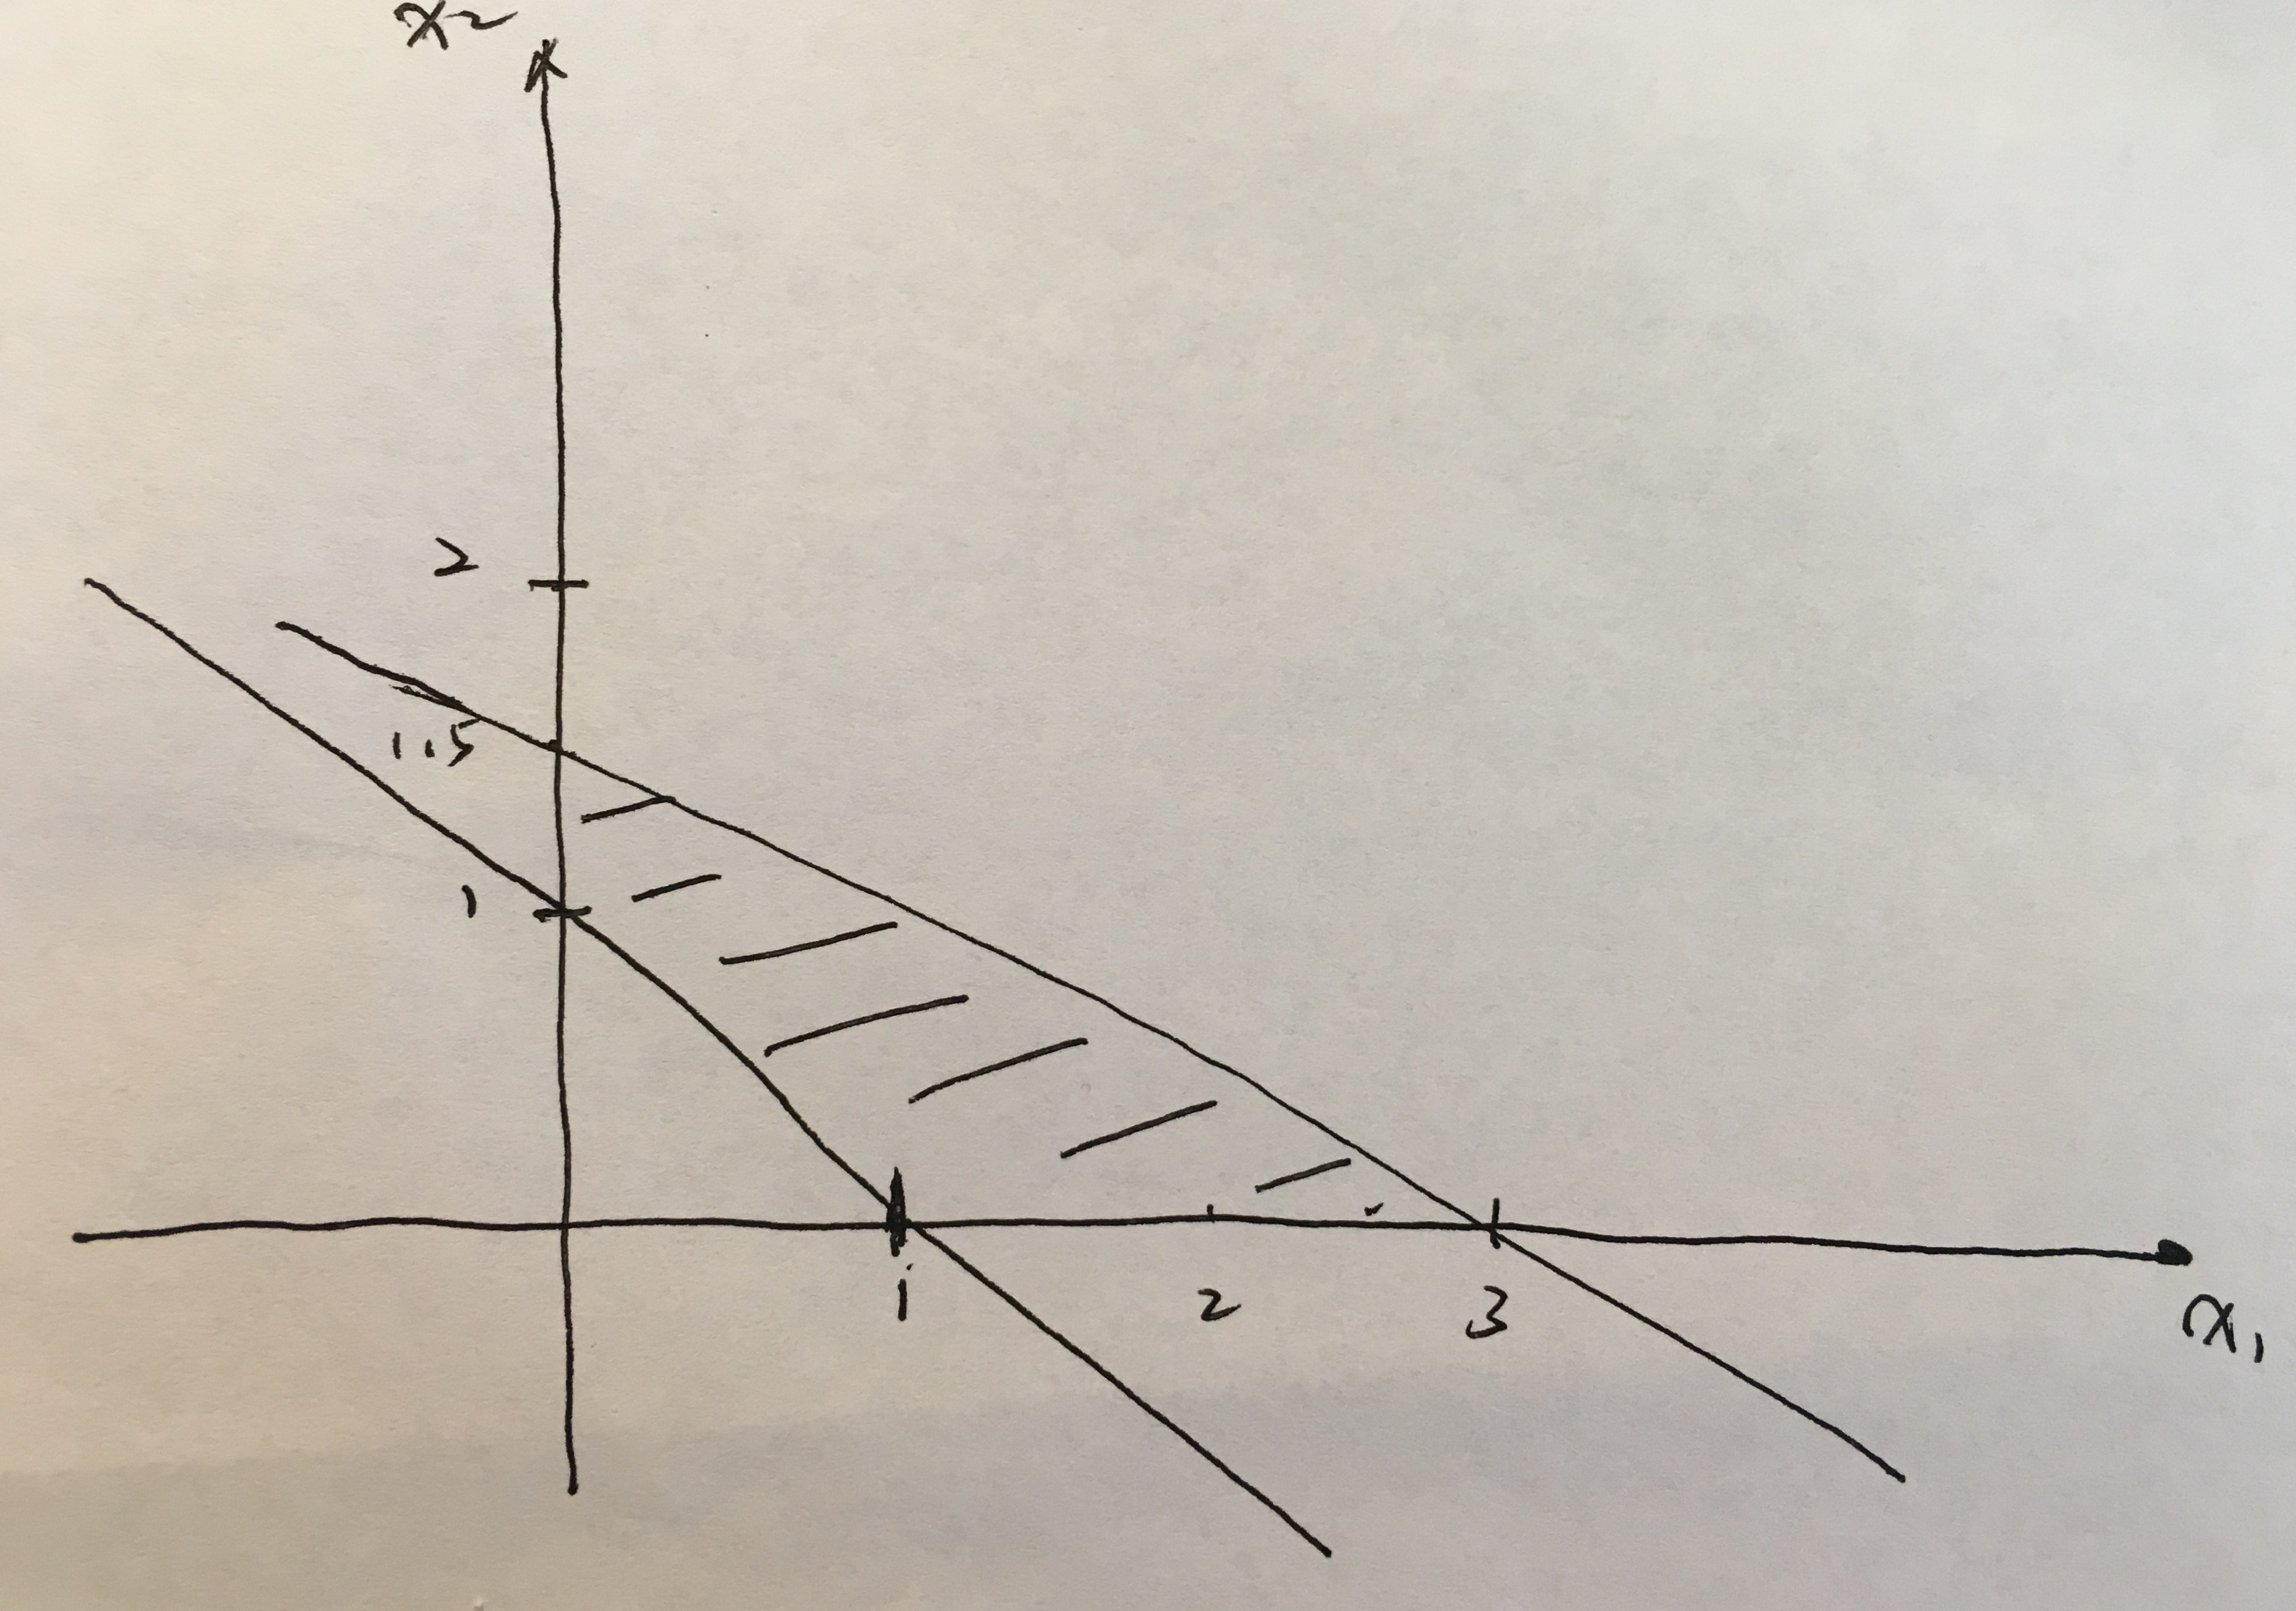
\includegraphics[width=0.7\textwidth]{2.jpg}
	\caption{Visualizing the constraints for $x_1$ and $x_2$ in the shaded area.}
	\label{fig:2}
\end{figure}
\paragraph{(a)} $c = (-1,0,0)$. 

The objective depends on $x_1$ only and minimize $-x_1$ we need to make $x_1$ as large as possible. Hence, as in Figure \ref{fig:2}, we can make $x_1$ = 3 by letting $x_2=0$. $x_3$ is dummy here, we only need it to be feasible, i.e. $x_3 \geq 0$. Therefore, the optimum value $cx = -3$ and the set of optimum solutions is $\{x | x_1 = 3, x_2 = 0, x_3 \geq0\}$.

\paragraph{(b)} $c = (0,1,0)$. 

The objective depends on $x_2$ only and minimize $x_2$ we need to make $x_2$ as small as possible. Hence, as in Figure \ref{fig:2}, we can make $x_2$ = 0 by letting $1 \leq x_1 \leq 3$. $x_3$ is again dummy here, we only need it to be feasible, i.e. $x_3 \geq 0$. Therefore, the optimum value $cx = 0$ and the set of optimum solutions is $\{x | 1 \leq x_1 \leq 3, x_2 = 0, x_3 \geq0\}$.

\paragraph{(c)} $c = (0,0,-1)$. 

The objective depends on $x_3$ only and minimize $-x_3$ we need to make $x_3$ as large as possible. However, notice that the \emph{only} constraint for $x_3$ is $x_3 \geq 0$, the problem is \emph{unbounded}. The `optimal' value can be $-\infty$, when $x_1$ and $x_2$ is in the shaded area in Figure \ref{fig:2} and $x_3=+\infty$. 

\newpage

\section*{Problem 3}
The idea is to divide the interval of $[-8, 8]$ for $c^Tx$ and solve the \emph{optimal} $f^Tx$ in each sub-interval. By `optimal' here we mean $maximum$ $f^Tx$ for positive $c^Tx$ sub-intervals and $minimum$ $f^Tx$ for negative $c^Tx$. Then we know the `true' optimum of the ratio in each sub-interval will be within $\{c^Tx\}_{left\:boundary} / f^T x$ and $\{c^Tx\}_{right\:boundary} / f^T x$. By dividing the sub-intervals fine enough, we can get arbitary precision $\epsilon$ for the optimal ratio. 
\paragraph{Algorithm} Divide the interval $[-8, 8]$ into $16/\epsilon$ sub-intervals, $[-8, -8 + \epsilon], [-8 + \epsilon, -8 + 2\epsilon], ~...., ~[8 - \epsilon, 8]$. Particularly, for the interval that contains $0$ inside, i.e. $0 \in [-8 + p\epsilon, -8 + (p+1)\epsilon]$ for some $p$, we further divide such sub-interval into two pieces, such that one only contains negative numbers the other only the positives.\footnote{Subdivision of interval for $0$ boundary should be considered for each analysis involving $[-8 + p\epsilon, -8 + (p+1)\epsilon]$, but omit hereafter for simplicity.} 

Then for each interval $[-8 + k\epsilon, -8 + (k+1)\epsilon]$, we use LP solver to solve the following LP problem, the objective switch to \emph{maximize} if the subinterval is positive and to \emph{minimize} if negative.
\begin{align*}
\text{maximize/minimize} &~f^Tx, \\
& Ax \geq b,\\
& f^Tx \geq 1,\\
& -8 + k\epsilon \leq c^Tx \leq -8 + (k+1)\epsilon.
\end{align*}
Notice that this LP problem can be transformed to standard/canonical form and thus a LP solver can be used as black box to solve for the optimal value. If the solver gives \emph{infeasible} return for \emph{each} sub-interval, the original problem is infeasible. For each feasible sub-interval, we compute\footnote{Return $0$ if the solver gives unbounded result, notice that the constraint $f^Tx \geq 1$ makes the unbounded direction $+\infty$ and this can only happens in the $\emph{maximize}$ case, which is when the sub-interval is positive.} $(c^Tx)/(f^Tx)$ and return with the minimum one as the result. 

\paragraph{Analysis} We now show the return has an additive error of $\pm\epsilon$. Denote the return $(c^Tx)/(f^Tx)$ in each interval as $\big\{(c^Tx)/(f^Tx)\big\}_{return}$. The true minimum of $(c^Tx)/(f^Tx)$ in each interval as $\big\{(c^Tx)/(f^Tx)\big\}_{true}$. Then we know, for each interval $[-8 + k\epsilon, -8 + (k+1)\epsilon]$
\begin{align*}
\frac{-8 + k\epsilon}{f^Tx} &\leq \big\{(c^Tx)/(f^Tx)\big\}_{return} \leq \frac{-8 + (k+1)\epsilon}{f^Tx},\\
\frac{-8 + k\epsilon}{f^Tx} &\leq \big\{(c^Tx)/(f^Tx)\big\}_{true} \leq \frac{-8 + (k+1)\epsilon}{f^Tx}.
\end{align*}
Therefore\footnote{There is a subtly that two return value can be off the true value by $2\epsilon$. This issue can be addressed by dividing the interval twice more frequent, which won't affect the LP solver using times in $O(\cdot)$ sense, and bound the analysis more rigorously.}, 
\begin{align*}
\big\{(c^Tx)/(f^Tx)\big\}_{true} - \epsilon &\leq \big\{(c^Tx)/(f^Tx)\big\}_{return} \leq \big\{(c^Tx)/(f^Tx)\big\}_{true} +\epsilon.
\end{align*}
By returning the minimum of all sub-interval, we have a result within the additive error $\epsilon$.

With the additional division of the interval containing $0$, the number of invoking LP solver is $O(16/\epsilon + 1) = O(\epsilon^{-1})$.

\newpage

\section*{Problem 4}
\paragraph{(a)}
The linear program can be formulated as follows\footnote{For simplicity, the formulation below represents \emph{an example}, and the general case is described as text.}. Specifically, the column vector denotes $[v_1, v_2, ..., ..., v_n]^T$ denotes the \emph{actual} transactions for $n$ clients, and $u_i$'s for their maximum amount of currency the client willing $i$ is willing to convert. The vector $[-D, 0, ..., 0]^T$ denotes all kinds of currency, and \emph{Dollar} is in the first entry, \emph{Yen} is in the second (thus the corresponding objective). 

The first matrix in the constraints is the `incoming' currency from each client. In particular, each row is for each currency, and the non-zero entries correspond to the amount those clients exchange in. The second matrix is the `outgoing' currency to each client and the non-zero entries denote the corresponding amount the clients will get in exchange. 

As the example shown below, for client $1$, $a_1$ is \emph{Dollar} and $b_1$ is \emph{Yen}, and she exchanges $r_1 v_1$ amount of $Yen$ for $v_1$ amount of \emph{Dollar}. Another example, client $2$ and client $n$ want to exchange in $v_2$ and $v_n$ amount of \emph{Dollar}, respectively; and client $2$ wants \emph{Yan} and $n$ wants the last currency for exchange, respectively. 
 
\begin{align*}
\text{maximize} ~ 
\begin{bmatrix}
r_1 & 0 & \dots & \dots & 0 \\
\end{bmatrix}
\begin{bmatrix}
v_1\\
v_2\\
\vdots\\
\vdots\\
v_n
\end{bmatrix} - 
\begin{bmatrix}
0 & 1 & \dots & \dots & 0 \\
\end{bmatrix}
\begin{bmatrix}
v_1\\
v_2\\
\vdots\\
\vdots\\
v_n
\end{bmatrix}\\ 
\text{subject to} ~
\begin{bmatrix}
	0 & r_2 & \dots & \dots & r_n \\
	r_1 & 0 & \dots & \dots & 0 \\
	\vdots & \vdots & \vdots & \ddots & \vdots \\
	0 & 0 & \dots & \dots & 0 \\
\end{bmatrix}
\begin{bmatrix}
v_1\\
v_2\\
\vdots\\
\vdots\\
v_n
\end{bmatrix} - 
\begin{bmatrix}
1 & 0 & \dots & \dots & 0 \\
0 & 1 & \dots & \dots & 0 \\
\vdots & \vdots & \vdots & \ddots & \vdots \\
0 & 0 & \dots & \dots & 1 \\
\end{bmatrix} 
\begin{bmatrix}
v_1\\
v_2\\
\vdots\\
\vdots\\
v_n
\end{bmatrix} &\geq 
\begin{bmatrix}
-D\\
0\\
\vdots\\
0
\end{bmatrix} \\
\begin{bmatrix}
v_1\\
v_2\\
\vdots\\
\vdots\\
v_n
\end{bmatrix}  \leq 
\begin{bmatrix}
u_1\\
u_2\\
\vdots\\
\vdots\\
u_n
\end{bmatrix} &
\end{align*}
The first constraint ensures that the company is able to give back the money it borrows for the transcations. The positive term is amount of money flows into the company, and second negative term is the amount that has to go out to the clients. $-D$ denotes that the company can potentially inject $D$ dollars for the transcations. The second constraint makes sure the transcations on clients don't exceed their limit. 

The objective says the company wants as much \emph{net} flow of \emph{Yen} as possible. (In this example, \emph{Yen} is the second currency.)

\paragraph{(b)} Notice that the solution from this linear program can be made acyclic. First, notice that there is no chance to make a profit by arbitrage, as provided as an assumption. Also, going around any directed cycle of trades, $\prod_i ri < 1$, this means we should \emph{not} perform a cycle of trades \emph{ever} as it loses the money. Therefore, it is possible to starts just with the $D$ Dollars and uses the money earned to perform further trades, as all cyclic trades won't be step in and all trades involved in the solution will be \emph{connected} with \emph{Dollar}.

\paragraph{(c)} We denote $Y$ as the optimal amount of \emph{Yen} we can achieve from (a). Then we construct another linear program with a slightly different constraint. 

\begin{align*}
\text{minimize} ~ 
\begin{bmatrix}
0 & r_2 & \dots & \dots & r_n \\
\end{bmatrix}
\begin{bmatrix}
v_1\\
v_2\\
\vdots\\
\vdots\\
v_n
\end{bmatrix} - 
\begin{bmatrix}
1 & 0 & \dots & \dots & 0 \\
\end{bmatrix}
\begin{bmatrix}
v_1\\
v_2\\
\vdots\\
\vdots\\
v_n
\end{bmatrix}\\ 
\text{subject to} ~
\begin{bmatrix}
r_1 & 0 & \dots & \dots & 0 \\
\vdots & \vdots & \vdots & \ddots & \vdots \\
0 & 0 & \dots & \dots & 0 \\
\end{bmatrix}
\begin{bmatrix}
v_1\\
v_2\\
\vdots\\
\vdots\\
v_n
\end{bmatrix} - 
\begin{bmatrix}
0 & 1 & \dots & \dots & 0 \\
\vdots & \vdots & \vdots & \ddots & \vdots \\
0 & 0 & \dots & \dots & 1 \\
\end{bmatrix} 
\begin{bmatrix}
v_1\\
v_2\\
\vdots\\
\vdots\\
v_n
\end{bmatrix} &=
\begin{bmatrix}
Y\\
\vdots\\
0
\end{bmatrix} \\
\begin{bmatrix}
v_1\\
v_2\\
\vdots\\
\vdots\\
v_n
\end{bmatrix}  \leq 
\begin{bmatrix}
u_1\\
u_2\\
\vdots\\
\vdots\\
u_n
\end{bmatrix} &
\end{align*}
This makes sure that we achieve the optimal \emph{Yen} while leave with no other currency. This is feasible because otherwise (a) could have obtained a larger \emph{Yen} by spending \emph{Dollars} on more trades leading to \emph{Yen}. \emph{Yen} here would not be smaller as well, because we only deduct the trades flowing to \emph{other} currency, if this leads to a smaller \emph{Yen} it means we uses \emph{Yen} in (a) to purchase other currency, which is sub-optimal. The objective here is actually redundent and should be \emph{automatically} reinforced, as it uses smallest amount of \emph{Dollars} to get the most \emph{Yen} (by not spending \emph{Dollars} on unrelated trades). 

\section*{Problem 5}
\paragraph{(a)} Notice that the two types of constraint include $n$ outgoing edge constraints $\sum_{j\in N(i)}x_{ij} = 1$ and $n$ incoming edge constraints $\sum_{i\in N(j)}x_{ij} = 1$. Also, notice that these $2n$ constraints are \emph{not} linearly independent. Because sum of all outgoing flows on one set of vertices equals to the sum of all incoming flows on the other set of the vertices, namely $\sum_i\sum_{j\in N(i)}x_{ij} = \sum_j\sum_{i\in N(j)}x_{ij}$, as the conservation of the flow. Therefore, there is only $2n-1$ linearly independent constraints. 

In vertex matrix $M$,  each entry denotes the connectivity between nodes, and there are $m$ entries. Also, the polytope of constraints form a hyper-plane. The $0$'s in the matrix correspond to each of the linear dependency. Therefore there are at least $m-2n+1$ entires filled up with $0$ in the matrix.

\paragraph{(b)} Notice that there are $n$ rows and $n$ columns in matrix $M$. For the $n$ rows, each denote the edges outgoing from the node. There has to be at least one entry being non-zero, otherwise no flow is going out from such a node, contradicts with bipartite matching. Recall in (a) that at most $2n-1$ entries in $M$ is non-zero and here we already `used' $n$ of them. The remaining $n-1$ non-zero values \emph{must} leave at least one row uncovered. In order words, there is at least one row only has one entry filled up with non-zero value. Since $\sum_{j\in N(i)}x_{ij} = 1$ and there is only one single value, we know the value has to be exactly $1$. 

Similar argument can be applied to column case and there must be at least one column that only has $1$ in one of the entries and $0$ the rest.  

\paragraph{(c)} We show the convex combination by decomposing the matrix into basis vertex matrix $M$'s one at a time. From matrix $M$, we create matrix $M_1$ that contains one entry from $M$'s each column and each row. Note that $M_1$ is a integral doubly stochastic matrix. Then we multiply $M_1$ with the smallest entires $\lambda_1$ and subtract $\lambda_1M_1$ from $M$. Notice that $M-\lambda_1M_1$ \emph{still} preserves the property that all row sums and all columns sums are equal. In order words, the two constraints for incoming and outgoing links only change the constant $1$ to some other quantity $1-\lambda_1$. The above analysis still hold (just to change the constant in the procedure). Then we can iterate the procedure to eliminate $M$ by a series of integral doubly stochastic matrix $M_1, M_2, ..., M_k$ with factor $\lambda_1, \lambda_2, ..., \lambda_k$. We know each operation takes out at least one entry (because the factor cancels the smallest element(s) in $M$), therefore the operations are finite. The above induction procedures give us perfect matching decomposition of $M$ with integral doubly stochastic matrix $M_1, M_2, ..., M_k$. Also, $\sum_i \lambda_i = 1$, because we can focus on a specific row (or column) in original $M$, each time $M_i$ takes out part of some entry in the row by $\lambda_i$ and all $M_i$'s exactly eliminate all quantities in the row. Since the sum of the row originally in $M$ is 1, we know $\sum_i \lambda_i = 1$.

For the Internet switching problem, as in the given example, two input lines $i_1$, $i_2$ and two output lines $o_1$, $o_2$. In a given time interval $i_1$ has 2 packets to send to $o_1$, and $i_2$ has one packet to send to $o_1$ and one packet to send to $o_2$. Then $i_1$, $i_2$ have rate 2 each, $o_1$ has rate 3 and $o_2$ has rate 1, hence $\lambda$ is 3. Notice that here the input rate and output rate is \emph{not} independent.To deliver all 4 packets using 3 matchings suffice (as opposed to 4 trivial matchings). One possible 3 matchings can be (1) $i_1 \to o_1$, $i_2 \to o_2$ (2) $i_1 \to o_1$ (3) $i_2 \to o_1$. The key observation here is that proper matching packs concurrent flow from inputs to outputs and makes the bottleneck at $\lambda$. 

In general, the above decomposition of perfect matchings gives us an procedure of matching and delivering Integer packets. Specifically, each time we carry out the above elimination of one entry from $M$'s each column and each row, where $M$ denotes the packet routing, with their rates. We take out $\lambda_i$ of $M_i$ (0-1 matrix denoting matching of in-out packets) and $\lambda_i$ means the \emph{lowest} rate (correspond to the smallest entry). The meaning for $\lambda_iM_i$ is that we are able to perform $\lambda_i$ packet routing according to the matching rule in $M_i$ in a unit of time (for the example above, this will be one of the three matching). We can keep this procedure until all packets are delivered. In the intermediate steps, some ports will be idle and have no packets to deliver, as in (2) $i_2$ and (3) $i_1$ in the above example. In these cases, we set the corresponding entry in $M_i$ to be 0. Notice that at the end $\sum_i \lambda_i = \lambda$ as it is the maximum rate in the input and output port (thus will appear in each elimination of $\lambda_iM_i$). Therefore so long as the switch can deliver matchings at rate $\lambda$, it can deliver the specified traffic.
\end{document}